\chapter{Flight Test Images}

\begin{figure}
  \centering
  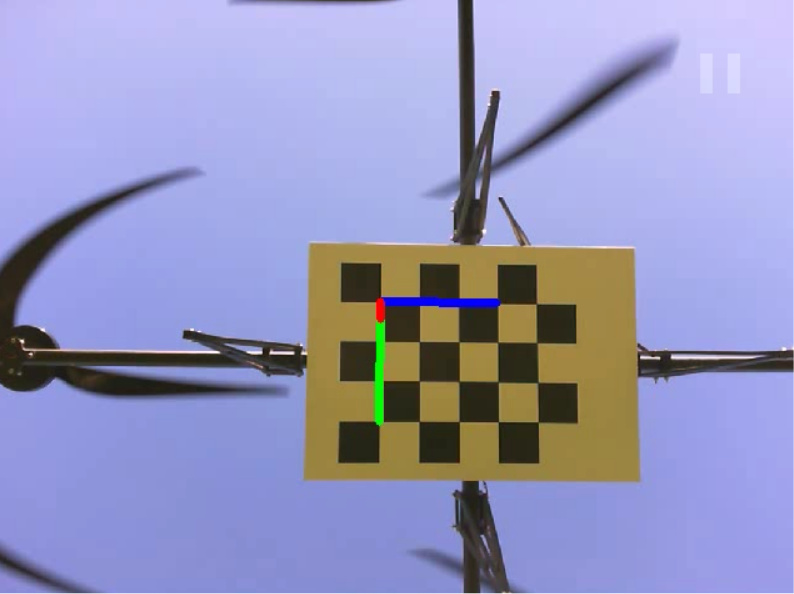
\includegraphics[width=\textwidth]{figures/appendices/oov2}
  \caption{Picture of a typical test image where the CVS drew an axis system on the board.}
\end{figure}

\begin{figure}
  \centering
  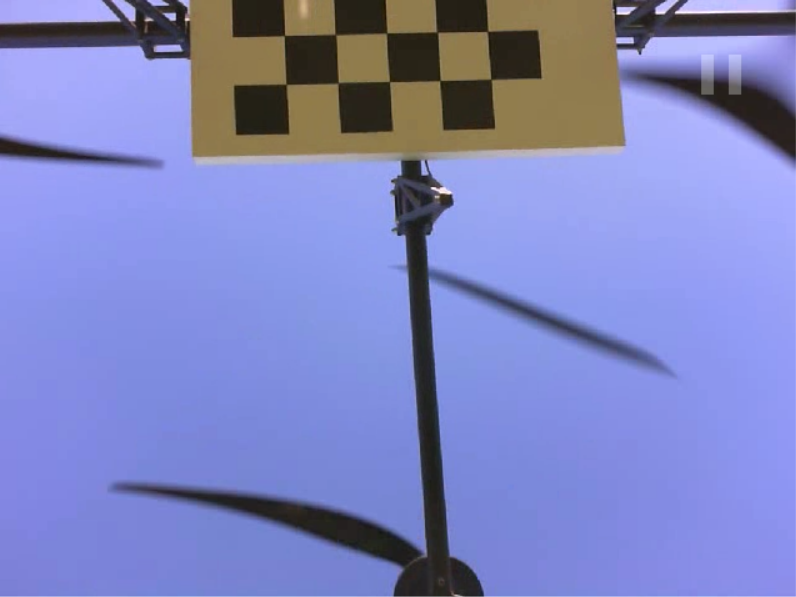
\includegraphics[width=\textwidth]{figures/appendices/oov1}
  \caption{Picture of where the board is partially out of the camera's view. The CVS could not capture all the corner data it required and could not draw an axis system on the board.}
\end{figure}

\begin{figure}
  \centering
  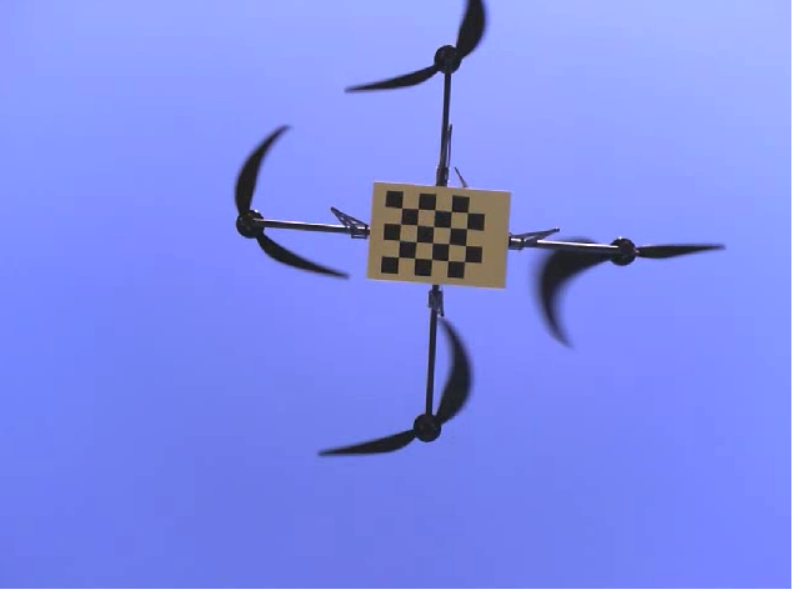
\includegraphics[width=\textwidth]{figures/appendices/oov4}
  \caption{Picture of where the board is too far away from the camera for the CVS to capture the corner data and draw an axis system.}
\end{figure}

\begin{figure}
  \centering
  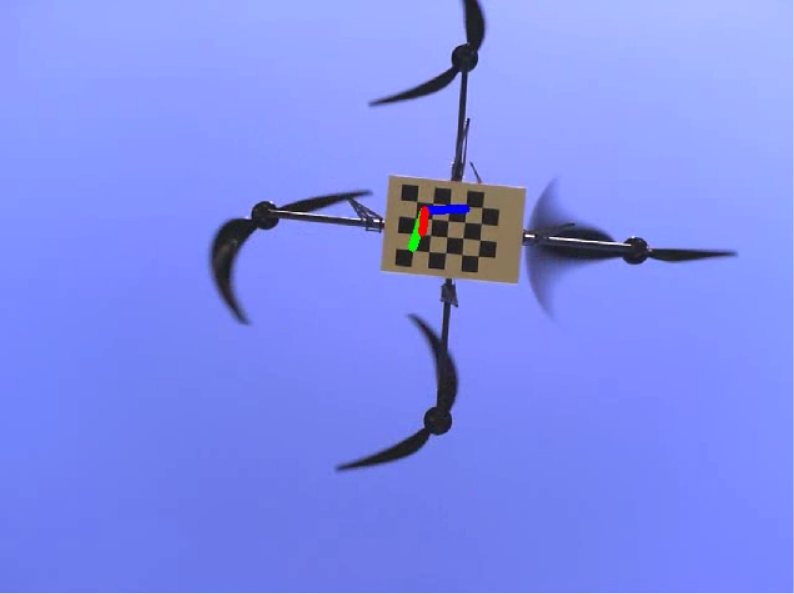
\includegraphics[width=\textwidth]{figures/appendices/oov7}
  \caption[Picture with an incorrect drawn axis system.]{Picture with an incorrect drawn axis system. Here, due to the board's distance from the camera and bad lighting conditions, the CVS could not accurately capture the corner information and drew an inaccurate axis system.}
\end{figure}

\endinput
